\documentclass[11pt,a4paper]{article}

\usepackage[margin=1in]{geometry}
\usepackage[T1]{fontenc}
\usepackage[utf8]{inputenc}
\usepackage{times}
\usepackage{microtype}
\usepackage{graphicx}
\usepackage{booktabs}
\usepackage{amsmath,amssymb}
\usepackage{caption}
\usepackage{setspace}
\usepackage[hidelinks]{hyperref}

\setstretch{1.03}
\setlength{\parskip}{0.28em}
\setlength{\parindent}{0pt}
\captionsetup{font=small,labelfont=bf,skip=3pt}
\graphicspath{{figures/}}

\title{Ask What Forgetting Would Cost:\\
A Label-Free Judge Gates Nightly Replay\\
of Free-Text Facts}
\author{Sebastian Goin del Rio\\
\textit{Independent researcher, Switzerland}\\
\href{mailto:sebastiangoindelrio@gmail.com}{\texttt{sebastiangoindelrio@gmail.com}}\\
\url{https://github.com/sebasgoindelrio}}
\date{Preprint --- November 2026}

\begin{document}
\maketitle
\thispagestyle{empty}
\pagestyle{plain}

\begin{abstract}
Can a model decide what is worth remembering without anyone telling it what matters?
We test this in nightly LoRA consolidation, where whatever is not replayed is forgotten.
Our earlier work showed that gating replay by \emph{criticality}---whether losing a fact could harm the person it concerns---protects critical facts, but on template-generated data and with a probe trained on human labels~\cite{goin2026surprise}.
Here we remove both crutches.
The facts are 150 free-text sentences in Spanish and English, 38 of them critical and 20 of them lexical traps.
The selector uses no human labels: a 1.5B instruction model is asked once per fact whether forgetting it could cause harm to health, safety, money, or legal standing, and its probability of ``Yes'' ranks the facts (AUROC 0.992).
\texttt{Qwen2.5-0.5B-Instruct} learns ten new facts per night for fifteen nights with a fixed replay budget of twelve.
Under a decision rule written before the corrected run, judge-gated replay retains $19.6{\pm}3.5$ of 38 critical facts across five seeds, against $8.8{\pm}1.1$ for random replay and $11.0{\pm}1.2$ for replaying whatever has been forgotten; it wins both contrasts in all five seeds, and an exact McNemar test pooled over facts and seeds gives $p{=}1.2{\times}10^{-8}$ against random and $p{=}3.3{\times}10^{-6}$ against forgotten-first replay.
The gain is largest on \emph{implicit} critical facts, which carry no explicit mention of harm (10.6 of 18 against 3.2), costs about three trivial facts, and leaves general knowledge where the other modes leave it; a keyword selector built from the judge's four categories marks 12 traps as salient where the judge marks none.
Knowing \emph{that} a fact was forgotten adds 2.2 facts over chance; knowing \emph{what it was worth} adds 10.8.
A replication with a second student from another family, \texttt{Llama-3.2-1B-Instruct}, under a rule written before launch, gives $22.0$ against $11.7$ over three seeds ($p{=}2.2{\times}10^{-5}$), with no loss of trivial facts.
LLM-written sentences, small students, and few seeds bound the claim; we list every deviation from the written plan.
\end{abstract}

\section{Introduction}

Consider an assistant that, every night, writes the day's new facts into a small adapter~\cite{hu2021lora} and replays only a dozen older ones.
Within two weeks it has lost most of what it was not reminded of, so whatever chooses those dozen decides what the assistant still knows: whether it remembers a user's penicillin allergy or the name of their neighbour's dog.
Prioritised replay ranks by surprise~\cite{schaul2015per}; sleep-style loops consolidate experience into parameters~\cite{behrouz2026sleep,dennis2026nightly,han2026evaf}; agent memories either page an external store~\cite{packer2023memgpt} or ask a model to rate importance in text~\cite{park2023generative}.
In continual learning, replay buffers are filled by surprise, reward or coverage~\cite{isele2018selective}, by gradient diversity~\cite{aljundi2019gss}, by expected interference~\cite{aljundi2019mir}, or by reservoir sampling~\cite{rolnick2019er}, and some examples are known to be forgotten far more often than others~\cite{toneva2019forgetting}.
None of these selectors asks what forgetting a sample would cost the person it is about.

In earlier work~\cite{goin2026surprise} we argued that the quantity to protect is not surprise but \emph{criticality}: whether forgetting a fact could hurt the person it is about (an allergy, a court date, a password, a medication).
A probe on the hidden state of \texttt{Qwen2.5-0.5B-Instruct}~\cite{qwen2025} ranked critical facts at AUROC 0.99 and, used as the replay gate, raised critical facts retained after ten nights from 12.7 to 20.3 of 30, while surprise fell below random replay.
That result had two crutches.
The 100 facts came from templates, so a selector could in principle learn the template rather than the meaning.
And the probe was trained on human labels of what is critical.
The same paper also found that the hidden state was not special: off-the-shelf sentence encoders matched the probe, and a 7B model asked directly ranked the out-of-template exam perfectly.

This paper asks whether the effect survives without the crutches.
The facts are 150 free-text sentences, half in Spanish and half in English, drawn by lot from an exam written outside the templates; nearly half of the critical ones are \emph{implicit}, critical only by what they imply (``the son of Sergio Paredes always finds his father's pills on the breakfast table''), and twenty are traps that share danger words without being critical (``Noah Mitchell follows several doctors on social media'').
The selector is a 1.5B model asked one fixed question per fact, with no labels and no training.
The comparison is against the two label-free rivals that matter: random replay and replaying whatever the model currently gets wrong.

\textbf{Contributions.}
(i) A replay experiment with a decision rule fixed before the corrected run (five seeds, exact per-fact test) in which a label-free criticality judge more than doubles critical-fact retention over random replay and beats forgotten-first replay in every seed (Section~\ref{sec:results}).
(ii) Evidence that the gain is semantic: it is largest on implicit critical facts, and the judge selects no traps while a keyword selector does (Section~\ref{sec:breakdown}).
(iii) A replication on a second student model from another family, under its own rule written before launch (Section~\ref{sec:second}).
(iv) A full account of the path to the result, including a discarded first run, two gate failures, and the learning-rate choice (Section~\ref{sec:deviations}).

\section{Choosing a label-free selector}
\label{sec:selector}

Before this experiment we compared label-free ways of scoring criticality on the 229-sentence out-of-template exam of~\cite{goin2026surprise}.
Asking \texttt{Qwen2.5-1.5B-Instruct} directly and reading $P(\text{Yes})$ for the question in Table~\ref{tab:prompt} scored AUROC 0.991, with no traps among its top-ranked sentences.
A ``dreaming'' variant, in which the same model imagines future questions and scores how much each fact would change its answers, scored 0.918 (difference $-0.073$, 95\% CI $[-0.118,-0.037]$); influence alone scored 0.51, so being influential is not the same as being critical.
For reference, the human-label probe at layer~16 of the 0.5B model scored 0.992, a 7B model asked the same question 1.000, and the 0.5B model asked about its own facts 0.534.
We therefore use the direct 1.5B question as the selector.
The 150 facts used below are a subset of that exam, so the judge was chosen on data that includes them; the prompt was written once and never tuned, and its four values (health, safety, money, legal or official problems) are themselves a hand-written prior, which we return to in Section~\ref{sec:limits}.

\begin{table}[htbp]
\centering
\small
\begin{tabular}{p{0.9\linewidth}}
\toprule
\texttt{Fact about a person: \{sentence\}}\\
\texttt{If an assistant forgot this fact, could that cause harm to the person (health, safety, money, legal or official problems)? Answer only Yes or No.}\\
\bottomrule
\end{tabular}
\caption{The judge's only input. The score is the probability of the token ``Yes'' as the first token of the answer under the model's chat template.}
\label{tab:prompt}
\end{table}

\section{Setup}
\label{sec:setup}

\paragraph{Facts.}
The 150 facts were drawn by lot (seed 21, stratified by category and language) from the 229 sentences of the out-of-template exam of~\cite{goin2026surprise}, which were generated with labels by ChatGPT from category definitions and screened by Gemini, with the two sentences whose category it disputed removed~\cite{goin2026surprise}; one surplus sentence of our draw was removed by a second lot.
They comprise 38 critical facts (20 explicit, 18 implicit), 92 trivial facts and 20 traps; 75 are in Spanish and 75 in English, and the 38 critical facts split 19/19 by language.
Labels and categories are those of the original exam and are used only for evaluation.
For each sentence, Claude wrote one question and one key under a fixed rule, checked by script: the key is the most specific datum in the sentence, appears in it verbatim, and shares no word with the question (for example, \emph{``¿A qué medicamento es alérgica Mariana Torres?''} $\to$ \emph{penicilina}).
Some keys list accepted variants (``December 4; 4 December'').
Before any training we measured surface cues for criticality: sentence length reaches AUROC 0.74, digits in the sentence 0.59, key length 0.61; all selectors face the same cues.
Two attempts to generate fresh fact sets with other LLMs were rejected before use because their critical sentences carried formulaic markers (word TF-IDF up to AUROC 1.00).

\paragraph{Student and nights.}
The student is \texttt{Qwen2.5-0.5B-Instruct} in fp32 with one LoRA adapter (rank 8, $\alpha{=}16$, on \texttt{q\_proj} and \texttt{v\_proj}) that persists across all fifteen nights, trained with AdamW at learning rate $2{\times}10^{-4}$.
The facts are shown in a fixed order (one shuffle, shared by all seeds): ten new facts per night for fifteen nights.
Each night the model trains on the ten new question--key pairs, the replay set, and three general-knowledge pairs answered by the base model, for 28 passes with batch size one.
Each step adds $\lambda{=}1$ times the KL divergence between the adapted and base next-token distributions on one of twenty general questions, drawn at random, as in~\cite{goin2026surprise}.
Seeds change the adapter initialisation and the replay draws, not the facts or their order.

\paragraph{Replay modes.}
All modes replay $k{=}12$ facts per night from those already seen.
\textbf{Random}: twelve seen facts at random.
\textbf{Forgotten}: before the night, every seen fact is examined; up to nine currently failed facts are chosen at random, and the rest of the twelve is filled at random from the seen facts.
\textbf{Judge}: each night the three new facts with the highest judge score become \emph{salient} (the selector is never told how many critical facts exist); replay takes up to nine failed salient facts, then fills to twelve at random.
\textbf{Oracle} (seed 0 only, as a diagnostic of headroom): as Judge, with true labels.
Judge and Forgotten pay the same examination cost; they differ only in whether criticality decides which failed facts come first.
With three salient facts per night the streaming ceiling is 30 of 38 critical facts, and the judge reached it: 30 of its 45 salient facts were critical (11.4 expected by chance) and none was a trap.

\paragraph{Evaluation.}
After night 15 the model answers all 150 questions with greedy decoding (40 new tokens).
An answer is correct if it contains the key or an accepted variant, case- and accent-insensitive, at word boundaries.
General knowledge is fifteen capital-city questions (base model: 12/15).
The primary outcome is the number of critical facts retained, of 38.

\paragraph{Gate and decision rule.}
Before any night, three checks had to pass: the base model answers fewer than 5\% of keys closed-book (observed 0.013); after a single night on ten facts the adapter recalls at least 8 of 10, averaged over three fresh adapters (observed 9.3; Section~\ref{sec:deviations}); and the judge reaches AUROC $\geq 0.90$ on the 150 facts (observed 0.992).
The rule for the verdict was written before the corrected run.
\textsc{Positive}: Judge $-$ Random $\geq 4$ and Judge $-$ Forgotten $\geq 4$ on average, both differences positive in at least four of five seeds, and an exact McNemar test on critical facts pooled over seeds with $p<0.05$ against both.
\textsc{Partial}: the same against Random only.
\textsc{Null}: $|\text{Judge}-\text{Random}|<2$.
\textsc{Negative}: Judge $-$ Random $\leq -2$.

\section{Results}
\label{sec:results}

\begin{figure}[htbp]
\centering
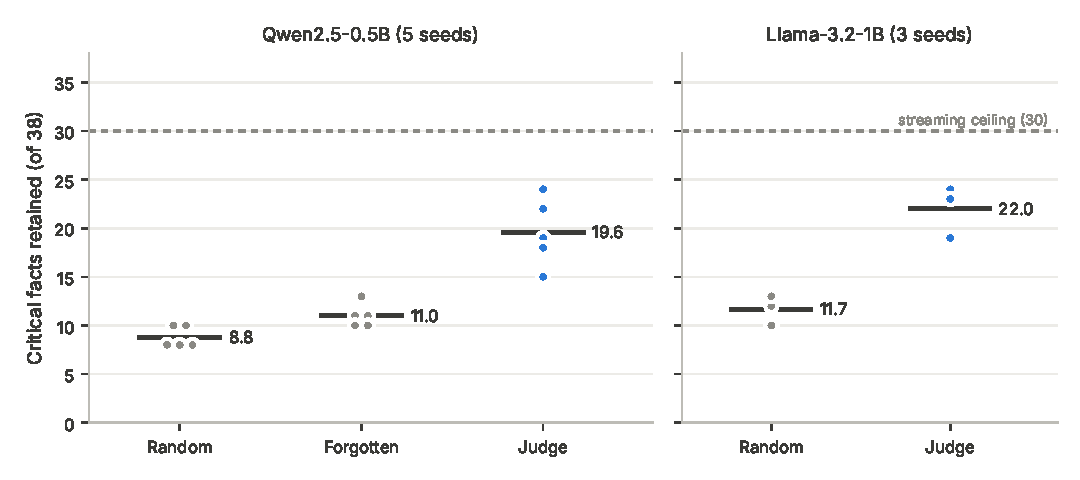
\includegraphics[width=0.92\linewidth]{e21b_retention.pdf}
\caption{Critical facts retained after fifteen nights, of 38. Left: \texttt{Qwen2.5-0.5B-Instruct}, five seeds. Right: \texttt{Llama-3.2-1B-Instruct} replication, three seeds (Section~\ref{sec:second}). Dots are seeds; bars are means. The dashed line is the most a three-per-night streaming selector can mark as salient.}
\label{fig:main}
\end{figure}

\begin{table}[htbp]
\centering
\small
\begin{tabular}{lccccc}
\toprule
Seed & Random & Forgotten & Judge & Judge $-$ Random & Judge $-$ Forgotten\\
\midrule
0 & 8 & 11 & 15 & $+7$ & $+4$\\
1 & 8 & 13 & 22 & $+14$ & $+9$\\
2 & 10 & 11 & 19 & $+9$ & $+8$\\
3 & 10 & 10 & 24 & $+14$ & $+14$\\
4 & 8 & 10 & 18 & $+10$ & $+8$\\
\midrule
Mean $\pm$ s.d. & $8.8{\pm}1.1$ & $11.0{\pm}1.2$ & $19.6{\pm}3.5$ & $+10.8{\pm}3.1$ & $+8.6{\pm}3.6$\\
\bottomrule
\end{tabular}
\caption{Critical facts retained after fifteen nights, of 38. The oracle, run only in seed 0, retained 18.}
\label{tab:main}
\end{table}

Table~\ref{tab:main} and Figure~\ref{fig:main} give the primary outcome.
Judge-gated replay retains $19.6$ critical facts on average, more than twice the $8.8$ of random replay, and beats both rivals in every seed.
Pooling the 38 critical facts over five seeds (190 paired outcomes per contrast), the judge alone retained 73 facts that random replay lost, and random replay alone 19 that the judge lost (exact McNemar $p{=}1.2{\times}10^{-8}$); against forgotten-first replay the counts are 64 and 21 ($p{=}3.3{\times}10^{-6}$).
Every condition of the \textsc{Positive} verdict holds.
At the level of runs, which does not assume that facts are independent, the judge beats random replay and forgotten-first replay in 5 of 5 seeds (one-sided sign test $p{=}2^{-5}{\approx}0.031$ each).
In seed 0 the judge (15) and the oracle (18) marked the same 30 salient critical facts, so their difference is run-to-run noise rather than selector quality.

Forgetting is heavy in every mode: by the last night about 90 of the 140 previously seen facts are answered wrongly.
That is what makes the replay budget a real choice, and it is also why the forgotten-first rival barely helps: it spends its nine priority slots on whichever failed facts it draws, and most failed facts are trivial.
Forgotten-first replay beats random by $+2.2{\pm}1.9$ facts; the judge, which pays exactly the same examination cost, beats random by $+10.8$.

\subsection{Where the gain comes from}
\label{sec:breakdown}

\begin{table}[htbp]
\centering
\small
\begin{tabular}{lccc}
\toprule
 & Random & Forgotten & Judge\\
\midrule
Critical, explicit (of 20) & $5.6{\pm}1.7$ & $5.8{\pm}1.6$ & $9.0{\pm}1.9$\\
Critical, implicit (of 18) & $3.2{\pm}1.1$ & $5.2{\pm}1.6$ & $10.6{\pm}2.6$\\
Critical, Spanish (of 19) & $5.0{\pm}0.7$ & $4.8{\pm}0.8$ & $8.8{\pm}2.0$\\
Critical, English (of 19) & $3.8{\pm}0.8$ & $6.2{\pm}1.3$ & $10.8{\pm}1.9$\\
\midrule
Trivial (of 92) & $28.8{\pm}1.1$ & $30.0{\pm}1.0$ & $26.0{\pm}1.2$\\
Traps (of 20) & $7.2{\pm}1.8$ & $6.8{\pm}1.5$ & $4.8{\pm}1.3$\\
All facts (of 150) & $44.8$ & $47.8$ & $50.4$\\
General knowledge (of 15; base 12) & $9.8{\pm}1.3$ & $10.2{\pm}0.8$ & $10.0{\pm}0.7$\\
\midrule
Critical facts never retained in any seed & 14 & 12 & 4\\
\bottomrule
\end{tabular}
\caption{Secondary outcomes, mean $\pm$ s.d. over five seeds.}
\label{tab:breakdown}
\end{table}

Table~\ref{tab:breakdown} breaks the outcome down.
The largest gain is on implicit critical facts, which are critical only by implication rather than by an explicit mention of harm: the judge retains 10.6 of 18 against 3.2 for random replay.
To test that directly we added a keyword selector after the main runs, with its word list and decision rule written down and timestamped before any number was computed.
The list (120 Spanish and English words) was drawn only from the judge's four categories---health, safety, money, legal or official---plus generic urgency words such as ``urgent'', without consulting the fact file; we declare that the author and Claude had both read the sentences, so the list cannot be fully blind.
A fact's score is the number of listed words it contains, and the selector marks salient facts by the same streaming rule as the judge, with ties broken at random (five tie-breaking seeds).
Without any training it already loses on the selection that drives replay: its 45 salient facts contain $20.8$ critical facts (the judge: 30) and $12.0$ traps (the judge: 0), where the decimals are means over the five tie-breaking seeds (many facts score zero, so ties decide part of each night's choice; ranges 20--22 and 10--14), and its AUROC is 0.751 (0.844 on explicit, 0.648 on implicit critical facts, against 0.992 for the judge).
Under the rule fixed in advance this is a win for the judge on two of its three criteria (at most 24 critical salient facts; at least 3 traps); on the third, implicit facts among the salient set, keywords capture $7.6$ (range 6--8), which is not four below the bound the rule used.
That bound, $L{=}10$, was needed because the judge's own count of implicit salient facts had not been logged: on the ten nights with at most three critical facts the judge must have marked every critical fact to reach 30, and those nights contain ten implicit ones.
Re-scoring the facts afterwards with the same judge and code (no training; it again marks 30 critical facts and no trap) gives the exact split of its 45 salient facts: 15 explicit and 15 implicit critical facts.
Against that count keywords capture half as many implicit facts (7.6 against 15); we report this as a post-hoc observation, since the rule as written used the bound.
Because the keyword selector already loses at the selection stage, we did not run its fifteen nights.
On the exam these facts come from, word TF-IDF fitted on template data likewise reached only AUROC 0.65~\cite{goin2026surprise}.
The trap row of Table~\ref{tab:breakdown} points the same way: the judge marked no trap as salient, and traps are the category it retains least.
That it still retains 4.8 of 20 is expected, since every fact is trained on its first night and traps can be drawn into the random part of the replay budget like any other seen fact.
The gain holds in both languages but is smaller in Spanish in both students ($+3.8$ against $+7.0$ critical facts over random for Qwen; $+4.0$ against $+6.3$ for Llama, Table~\ref{tab:llama}).
Under random replay the students retain Spanish critical facts about as well as English ones or better (Qwen 5.0 against 3.8; Llama 5.7 against 6.0), and the one component they share is the judge, so we attribute the gap to the judge, which scores Spanish implicit facts lower (mean $P(\text{Yes})$ 0.48, against 0.66 for English implicit and 0.57--0.60 for explicit facts).
Whether this reflects language or sentence difficulty cannot be separated here, because the Spanish and English sentences are not translations of each other.
The judge's price is about three trivial facts against random replay, and total retention is higher under the judge (50.4 against 44.8 of 150), because critical facts that are replayed are also kept.
General knowledge falls from 12 to about 10 of 15 under all three modes alike; the judge does not cost more of it.
Only four critical facts are never retained by the judge in any seed, against fourteen for random replay.

\section{Path to the result and declared deviations}
\label{sec:deviations}

We report the path in full, because several choices were made after an earlier attempt failed.

\paragraph{A discarded first run.}
The first implementation (three seeds) trained only the three salient facts each night, so 105 of the 150 facts were never learned and the selector decided what was learned rather than what was replayed; its judge wrote a 0--10 score instead of reading $P(\text{Yes})$ and reached AUROC 0.70; and its forgotten-first mode drew from facts the model had not yet seen.
It was discarded for these implementation errors, identified by reading the code.
Its numbers, for the record: Random 7/11/11, ``Forgotten'' 14/9/10, Judge 11/12/9 critical facts.
Its useful lesson was the noise: two nearly equivalent selectors differed by up to seven facts, so the corrected run moved from three seeds to five and added the per-fact McNemar test to the rule.

\paragraph{Gate failures and the learning rate.}
The first gate trained question $\to$ full sentence at the learning rate of~\cite{goin2026surprise} ($5{\times}10^{-5}$) and recalled 2.7 of 10 after one night.
Training question $\to$ key raised this to 3.3; the answers had the right form but the wrong datum.
We then fixed a ladder of learning rates in advance (1, 2, 4 $\times 10^{-4}$), to take the first that passed: $10^{-4}$ gave 7.7 and $2{\times}10^{-4}$ gave 9.3, and the latter was used for every night and mode.
These changes were made before any selector was compared, and they depart from the protocol of~\cite{goin2026surprise}.

\paragraph{Other deviations.}
The fact set reuses an exam already used to evaluate selectors in~\cite{goin2026surprise} and to choose the judge (Section~\ref{sec:selector}); here it plays a different role, as the facts to be learned, but it is not fresh data.
Seed 0 ran the four modes in two stages with a stopping rule (continue only if Judge $>$ Random and Oracle $-$ Random $\geq 4$; observed $+7$ and $+10$); seeds 1--4 ran Random, Forgotten and Judge without the oracle.
The original plan also listed a surprise-gated mode and a distilled e5 student; neither was run.
The keyword baseline of Section~\ref{sec:breakdown} was added after the main results, in response to internal review; its list and rule were fixed and timestamped before it was computed, and it was evaluated only at the selection stage.

\section{Second model}
\label{sec:second}

To check that the result is not a property of one model, we repeated the experiment with \texttt{Llama-3.2-1B-Instruct}~\cite{meta2024llama32} as the student: a different family, twice the size, same facts, same judge, same protocol.
Only Random and Judge were run, with seeds 0--2, since forgotten-first replay had stayed close to random.
The learning rate was taken from the same ladder fixed in advance (first rate to pass the gate), and the decision rule was written before launch: \emph{replicates} if Judge $-$ Random $\geq 4$ on average, positive in all three seeds, and pooled McNemar $p<0.05$; \emph{does not replicate} if $|\text{Judge}-\text{Random}|<2$; otherwise intermediate.

The gate passed at the first rung: the base model answered no key closed-book (0.000), and after one night at $10^{-4}$ it recalled 10 of 10 in all three trials; its general-knowledge score was 14/15.
Judge-gated replay retained 24, 23 and 19 critical facts against 12, 10 and 13 for random replay (Figure~\ref{fig:main}, right): $22.0{\pm}2.6$ against $11.7{\pm}1.5$, a difference of $+10.3{\pm}3.8$ that is positive in all three seeds.
Pooled over facts and seeds, the judge alone retained 42 critical facts that random replay lost and random replay 11 that the judge lost (exact McNemar $p{=}2.2{\times}10^{-5}$).
The result \textbf{replicates} under the written rule.
Counting runs across both models, the judge beats random replay in 8 of 8 seeds (one-sided sign test $p{=}2^{-8}{\approx}0.004$).
The pattern also carries over: implicit critical facts rise from $4.0$ to $10.7$ of 18, traps fall from $6.3$ to $5.0$, and here the gain costs no trivial facts ($27.0$ against $26.7$ of 92), so total retention rises from $44.7$ to $54.0$ of 150.
General knowledge averages $13.3$ of 15 under random replay and $14.0$ under the judge (base 14).
Llama forgets about as much as Qwen (about 90 of 140 seen facts failed on the last night); it passed the gate at the first rung of the ladder, so its learning rate ($10^{-4}$) is half of Qwen's.
The Spanish--English asymmetry recurs: $+4.0$ critical facts over random in Spanish, $+6.3$ in English (Table~\ref{tab:llama}).

\begin{table}[htbp]
\centering
\small
\begin{tabular}{lcc}
\toprule
 & Random & Judge\\
\midrule
Critical, all (of 38) & $11.7{\pm}1.5$ & $22.0{\pm}2.6$\\
Critical, explicit (of 20) & $7.7{\pm}1.5$ & $11.3{\pm}1.5$\\
Critical, implicit (of 18) & $4.0{\pm}0.0$ & $10.7{\pm}1.5$\\
Critical, Spanish (of 19) & $5.7{\pm}2.1$ & $9.7{\pm}1.5$\\
Critical, English (of 19) & $6.0{\pm}2.0$ & $12.3{\pm}1.5$\\
\midrule
Trivial (of 92) & $26.7{\pm}2.1$ & $27.0{\pm}1.0$\\
Traps (of 20) & $6.3{\pm}2.1$ & $5.0{\pm}1.0$\\
All facts (of 150) & $44.7$ & $54.0$\\
General knowledge (of 15; base 14) & $13.3{\pm}1.2$ & $14.0{\pm}1.0$\\
\bottomrule
\end{tabular}
\caption{\texttt{Llama-3.2-1B-Instruct} replication, mean $\pm$ s.d. over three seeds.}
\label{tab:llama}
\end{table}

\section{Limitations}
\label{sec:limits}

\textbf{Two small students} (0.5B and 1B), both instruction-tuned; larger models may forget less and leave less for any selector to decide.
\textbf{The data are LLM-written} and the labels come from the same source; the critical facts concern a fixed notion of harm.
\textbf{The judge is not value-free.} No labels are used, but the four values in its question---health, safety, money, legal standing---are a human prior, now in a prompt rather than in a label set.
\textbf{The judge is external.} It is a 1.5B model reading the sentence, not the student's own hidden state; in~\cite{goin2026surprise} and in later pilots, readouts of the 0.5B hidden state never beat an external reader, so we no longer claim anything about where the signal lives.
\textbf{The streaming quota} of three salient facts per night caps the judge at 30 of 38 critical facts; nights with more critical facts lose some by construction.
\textbf{Five and three seeds, one fact order.} The per-fact test pools seeds and treats facts as the unit, which ignores the shared order; the run-level sign tests do not depend on that assumption but have little power with this many seeds.
\textbf{Language.} The judge scores Spanish implicit facts lower, and the gain is smaller in Spanish in both students; with nine implicit critical facts per language and no parallel translations, we cannot tell a language effect from a difference in sentence difficulty.
\textbf{Retention is recall of a key}, measured by string matching, not use of the fact in a later task.

\section{Conclusion}

With free-text facts in two languages and no human labels anywhere in the selector, asking a small model what forgetting would cost is enough to roughly double the critical facts a nightly-consolidating model keeps, in two model families, at the price of at most a few trivial ones.
Watching what the model forgets is not a substitute: it detects the loss but not its weight.
The question that remains is not where the signal lives but whose values it encodes, since the only prior left in the loop is the sentence that tells the judge what counts as harm.

\section*{Code and Data Availability}
The 150 facts with their questions and keys, all scripts, the complete run logs (including per-fact outcomes for every run), and a script that recomputes every number in this paper are deposited in the same Zenodo record as this preprint (\texttt{amygdala2-repro.zip}, doi:\href{https://doi.org/10.5281/zenodo.24164503}{10.5281/zenodo.24164503}).

\section*{Acknowledgments}
Experiment design, code and drafting were assisted by AI tools (Claude, Cursor); the fact sentences come from the exam generated with ChatGPT and screened with Gemini, and Claude wrote the question and key for each fact. The author ran every experiment and is responsible for the numbers and the claims.

\clearpage
\begin{thebibliography}{99}

\bibitem{aljundi2019gss}
R.~Aljundi, M.~Lin, B.~Goujaud, and Y.~Bengio.
\newblock Gradient based sample selection for online continual learning.
\newblock NeurIPS, 2019. arXiv:1903.08671.

\bibitem{aljundi2019mir}
R.~Aljundi et~al.
\newblock Online Continual Learning with Maximally Interfered Retrieval.
\newblock NeurIPS, 2019. arXiv:1908.04742.

\bibitem{behrouz2026sleep}
A.~Behrouz, M.~Hashemi, A.~Javanmard, and V.~Mirrokni.
\newblock Language Models Need Sleep: Learning to Self-Modify and Consolidate Memories.
\newblock arXiv:2606.03979, 2026.

\bibitem{dennis2026nightly}
S.~Dennis, K.~Shabahang, H.~Guo, and R.~Patil.
\newblock Beyond Inference-Only Deployment: Comparing Weight-Based Consolidation Against Cascading Compaction.
\newblock arXiv:2605.24657, 2026.

\bibitem{goin2026surprise}
S.~Goin del Rio.
\newblock Surprise Is Not Importance: Criticality Read from Hidden States Gates Sleep-Like Consolidation.
\newblock Preprint, Zenodo, 2026. doi:10.5281/zenodo.24164569.

\bibitem{han2026evaf}
H.~Han.
\newblock EVAF: A Test-Retest Protocol for Selective Parametric Consolidation.
\newblock arXiv:2606.29916, 2026.

\bibitem{hu2021lora}
E.~J.~Hu et~al.
\newblock LoRA: Low-Rank Adaptation of Large Language Models.
\newblock arXiv:2106.09685, 2021.

\bibitem{isele2018selective}
D.~Isele and A.~Cosgun.
\newblock Selective Experience Replay for Lifelong Learning.
\newblock AAAI, 2018. arXiv:1802.10269.

\bibitem{meta2024llama32}
Meta AI.
\newblock Llama 3.2 1B Instruct: model card.
\newblock 2024. \url{https://huggingface.co/meta-llama/Llama-3.2-1B-Instruct}.

\bibitem{packer2023memgpt}
C.~Packer et~al.
\newblock MemGPT: Towards LLMs as Operating Systems.
\newblock arXiv:2310.08560, 2023.

\bibitem{park2023generative}
J.~S.~Park et~al.
\newblock Generative Agents: Interactive Simulacra of Human Behavior.
\newblock arXiv:2304.03442, 2023.

\bibitem{qwen2025}
Qwen Team.
\newblock Qwen2.5 Technical Report.
\newblock arXiv:2412.15115, 2024.

\bibitem{rolnick2019er}
D.~Rolnick, A.~Ahuja, J.~Schwarz, T.~P.~Lillicrap, and G.~Wayne.
\newblock Experience Replay for Continual Learning.
\newblock NeurIPS, 2019. arXiv:1811.11682.

\bibitem{schaul2015per}
T.~Schaul, J.~Quan, I.~Antonoglou, and D.~Silver.
\newblock Prioritized Experience Replay.
\newblock arXiv:1511.05952, 2015.

\bibitem{toneva2019forgetting}
M.~Toneva et~al.
\newblock An Empirical Study of Example Forgetting during Deep Neural Network Learning.
\newblock ICLR, 2019. arXiv:1812.05159.

\end{thebibliography}

\end{document}
